\documentclass[11pt]{article}
\usepackage{fontspec}
\setmainfont{NotoSerif-Regular.ttf}[Path=C:/Windows/Fonts/,ItalicFont=NotoSerif-Italic.ttf,BoldFont=NotoSerif-Bold.ttf,BoldItalicFont=NotoSerif-BoldItalic.ttf]
\usepackage[a4paper,margin=22mm]{geometry}
\usepackage{amsmath,amssymb,graphicx,xcolor,hyperref,needspace,tikz}
\usepackage[normalem]{ulem}
\let\MathUnderline\underline
\renewcommand{\underline}[1]{\ifmmode\MathUnderline{#1}\else\uline{#1}\fi}
\hypersetup{unicode=true,colorlinks=true,linkcolor=blue,pdfauthor={}}
\setlength{\parindent}{0pt}
\setlength{\parskip}{.4em}
\setlength{\emergencystretch}{3em}
\raggedright
\newcommand{\SourcePage}[2]{\par\smallskip\phantomsection\label{#1:source-page}{\small\sffamily\color{blue!55!black}#1}\par\smallskip}
\newcommand{\EvidenceBlock}[4]{%
 \par\smallskip\noindent\begin{minipage}{\linewidth}
 \begin{minipage}[t]{.47\linewidth}\vspace{0pt}\centering
 \csname evidence-#1-#2\endcsname\par
 {\scriptsize\SourceCropCaption\ #1}\par
 \end{minipage}\hfill
 \begin{minipage}[t]{.49\linewidth}\vspace{0pt}\raggedright
 {\small\color{orange!65!black}\textbf{#4} #3}\par
 \end{minipage}
 \end{minipage}\par\smallskip}
\newcommand{\Unclear}[3]{\EvidenceBlock{#1}{#2}{#3}{\ReadingCaption}}
\newcommand{\Incomplete}[3]{\EvidenceBlock{#1}{#2}{#3}{\IncompleteCaption}}
\newcommand{\SourceFigure}[3]{\EvidenceBlock{#1}{#2}{#3}{\DiagramCaption}}
\expandafter\def\csname evidence-GELFAND-P000001-module-letter\endcsname{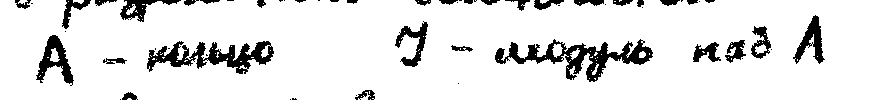
\includegraphics[width=\linewidth]{figures/gelfand-p000001-module-letter-original.png}}
\expandafter\def\csname evidence-GELFAND-P000001-diagram-blowup\endcsname{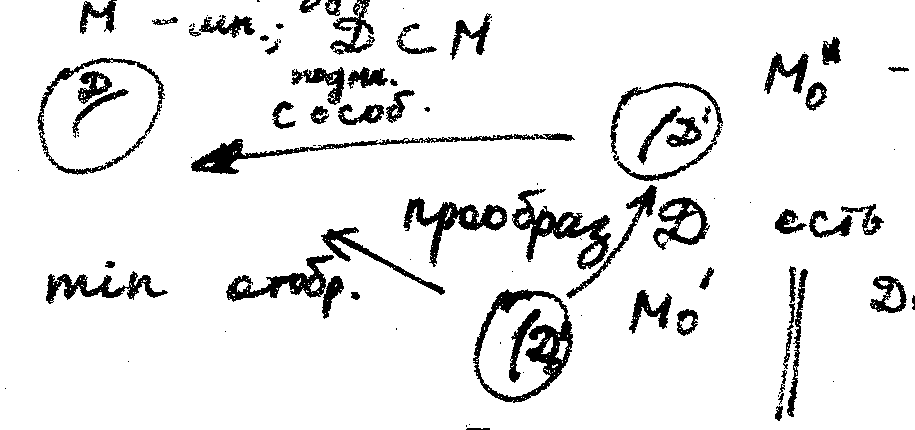
\includegraphics[width=\linewidth]{figures/gelfand-p000001-diagram-blowup-original.png}}
\expandafter\def\csname evidence-GELFAND-P000001-blowup-notation\endcsname{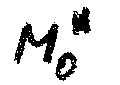
\includegraphics[width=.43\linewidth]{figures/gelfand-p000001-upper-blowup-label-original.png}\hfill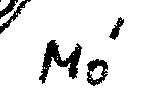
\includegraphics[width=.50\linewidth]{figures/gelfand-p000001-lower-blowup-label-original.png}}
\expandafter\def\csname evidence-GELFAND-P000001-origin-example\endcsname{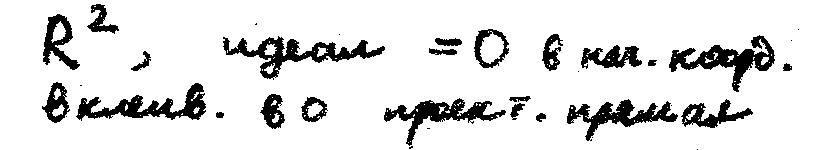
\includegraphics[width=\linewidth]{figures/gelfand-p000001-origin-example-original.png}}
\newcommand{\SourceCropCaption}{Original source details:}\newcommand{\ReadingCaption}{Uncertain reading.}\newcommand{\IncompleteCaption}{Undeciphered passage.}\newcommand{\DiagramCaption}{Diagram and typed description.}
\hypersetup{pdftitle={Gelfand seminar — chapter 1}}

\expandafter\def\csname evidence-GELFAND-P000002-ideal-selection\endcsname{
\includegraphics[width=\linewidth]{figures/gelfand-p000002-ideal-selection-part01-original-r1.png}}
\expandafter\def\csname evidence-GELFAND-P000002-open-set-notation\endcsname{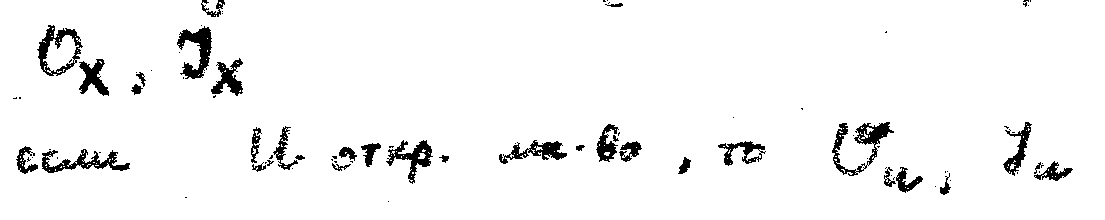
\includegraphics[width=\linewidth]{figures/gelfand-p000002-open-set-notation-part01-original-r2.png}}
\expandafter\def\csname evidence-GELFAND-P000002-fractions-sentence\endcsname{
\includegraphics[width=\linewidth]{figures/gelfand-p000002-fractions-sentence-part01-original-r1.png}\par\smallskip
\includegraphics[width=\linewidth]{figures/gelfand-p000002-fractions-sentence-part02-original-r1.png}\par\smallskip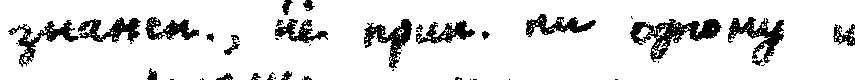
\includegraphics[width=\linewidth]{figures/gelfand-p000002-fractions-sentence-part03-original-r1.png}\par\smallskip
\includegraphics[width=\linewidth]{figures/gelfand-p000002-fractions-sentence-part04-original-r1.png}}
\expandafter\def\csname evidence-GELFAND-P000002-margin-grothendieck\endcsname{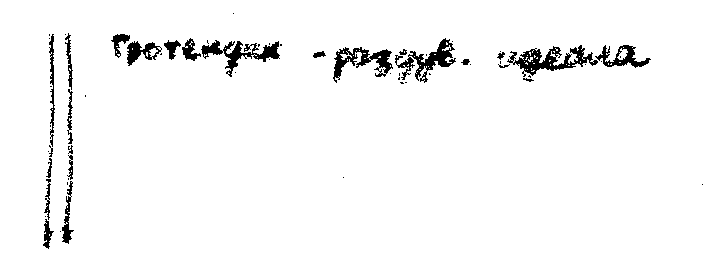
\includegraphics[width=\linewidth]{figures/gelfand-p000002-margin-grothendieck-part01-original-r1.png}}
\expandafter\def\csname evidence-GELFAND-P000002-quadratic-coefficients\endcsname{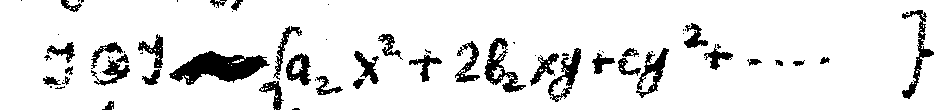
\includegraphics[width=\linewidth]{figures/gelfand-p000002-quadratic-coefficients-part01-original-r1.png}}
\expandafter\def\csname evidence-GELFAND-P000002-last-sign\endcsname{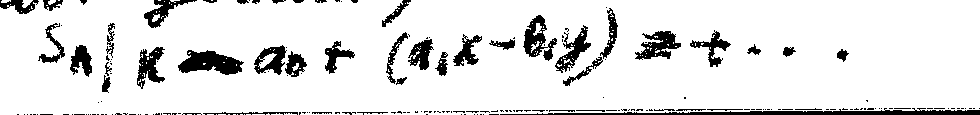
\includegraphics[width=\linewidth]{figures/gelfand-p000002-last-sign-part01-original-r1.png}}
\expandafter\def\csname evidence-GELFAND-P000003-directions\endcsname{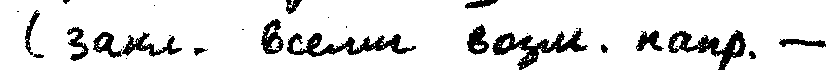
\includegraphics[width=\linewidth]{figures/gelfand-p000003-directions-part01-original-r1.png}\par\smallskip
\includegraphics[width=\linewidth]{figures/gelfand-p000003-directions-part02-original-r1.png}}
\expandafter\def\csname evidence-GELFAND-P000003-cross-cancellation\endcsname{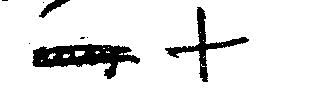
\includegraphics[width=\linewidth]{figures/gelfand-p000003-cross-cancellation-part01-original-r1.png}}
\expandafter\def\csname evidence-GELFAND-P000003-ising-cancellation\endcsname{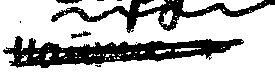
\includegraphics[width=\linewidth]{figures/gelfand-p000003-ising-cancellation-part01-original-r1.png}}
\expandafter\def\csname evidence-GELFAND-P000003-configuration-letter\endcsname{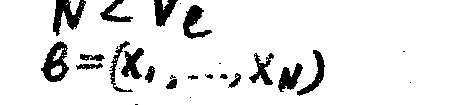
\includegraphics[width=\linewidth]{figures/gelfand-p000003-configuration-letter-part01-original-r2.png}}
\expandafter\def\csname evidence-GELFAND-P000003-energy-cancellation\endcsname{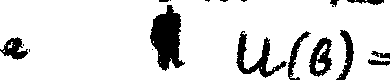
\includegraphics[width=\linewidth]{figures/gelfand-p000003-energy-cancellation-part01-original-r1.png}}
\expandafter\def\csname evidence-GELFAND-P000003-energy-case\endcsname{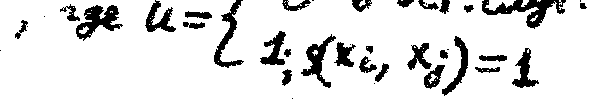
\includegraphics[width=\linewidth]{figures/gelfand-p000003-energy-case-part01-original-r2.png}\par\smallskip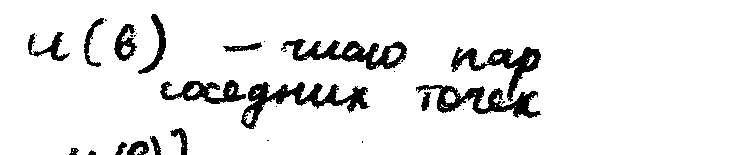
\includegraphics[width=\linewidth]{figures/gelfand-p000003-energy-case-part02-original-r3.png}}
\expandafter\def\csname evidence-GELFAND-P000003-partition-domain\endcsname{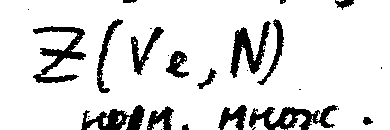
\includegraphics[width=\linewidth]{figures/gelfand-p000003-partition-domain-part01-original-r1.png}\par\smallskip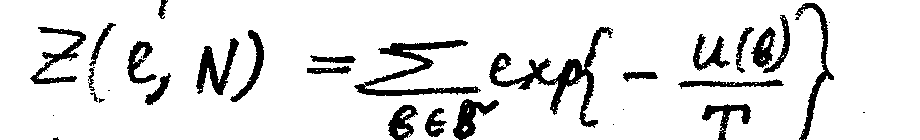
\includegraphics[width=\linewidth]{figures/gelfand-p000003-partition-domain-part02-original-r1.png}}
\expandafter\def\csname evidence-GELFAND-P000003-attraction-note\endcsname{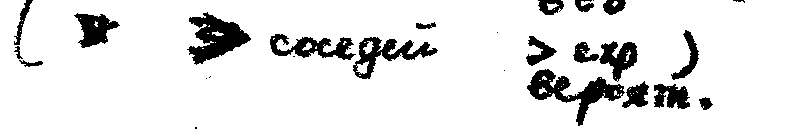
\includegraphics[width=\linewidth]{figures/gelfand-p000003-attraction-note-part01-original-r1.png}}
\expandafter\def\csname evidence-GELFAND-P000003-density-cancellation\endcsname{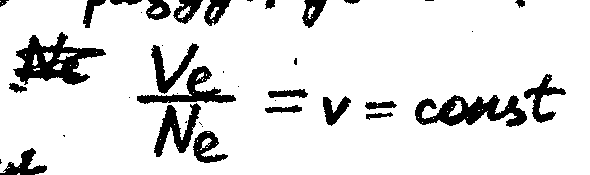
\includegraphics[width=\linewidth]{figures/gelfand-p000003-density-cancellation-part01-original-r1.png}}

\expandafter\def\csname evidence-GELFAND-P000004-pressure-letter\endcsname{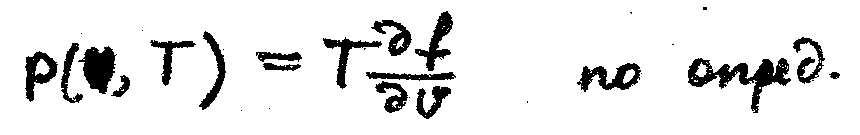
\includegraphics[width=\linewidth]{figures/gelfand-p000004-pressure-letter-part01-original-r1.png}}
\expandafter\def\csname evidence-GELFAND-P000004-diagram-phase-point\endcsname{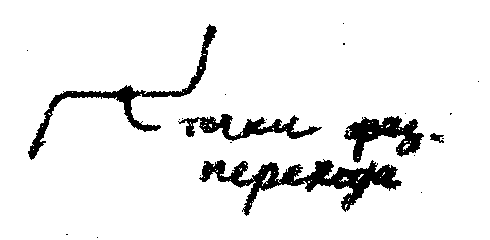
\includegraphics[width=\linewidth]{figures/gelfand-p000004-diagram-phase-point-part01-original-r2.png}}
\expandafter\def\csname evidence-GELFAND-P000004-diagram-cancelled-graph\endcsname{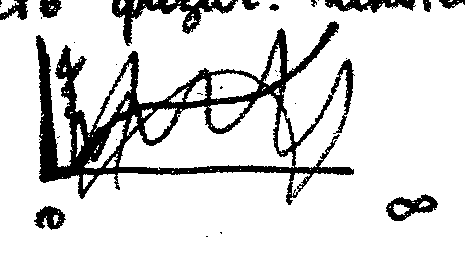
\includegraphics[width=\linewidth]{figures/gelfand-p000004-diagram-cancelled-graph-part01-original-r1.png}}
\expandafter\def\csname evidence-GELFAND-P000004-diagram-onsager\endcsname{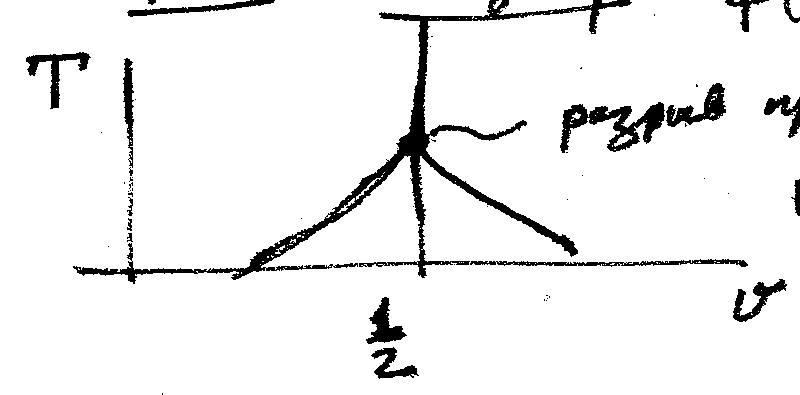
\includegraphics[width=\linewidth]{figures/gelfand-p000004-diagram-onsager-part01-original-r1.png}}
\expandafter\def\csname evidence-GELFAND-P000004-kac-helfand-note\endcsname{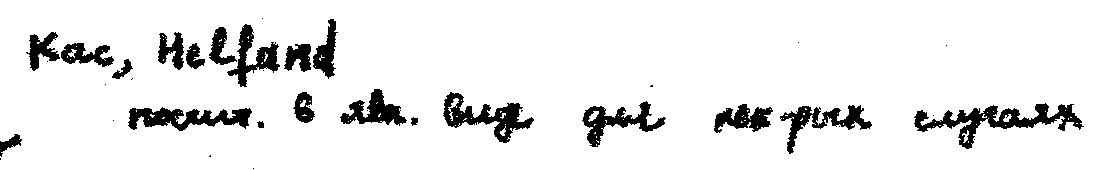
\includegraphics[width=\linewidth]{figures/gelfand-p000004-kac-helfand-note-part01-original-r1.png}}
\expandafter\def\csname evidence-GELFAND-P000004-diagram-subcube\endcsname{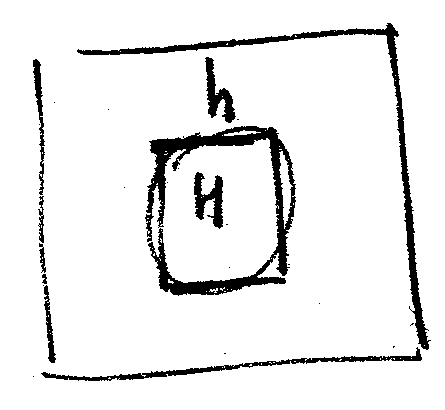
\includegraphics[width=\linewidth]{figures/gelfand-p000004-diagram-subcube-part01-original-r1.png}}
\expandafter\def\csname evidence-GELFAND-P000004-probability-bar\endcsname{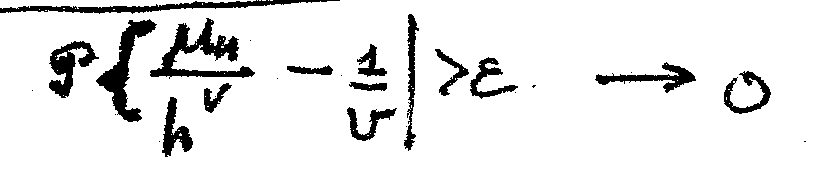
\includegraphics[width=\linewidth]{figures/gelfand-p000004-probability-bar-part01-original-r1.png}}
\expandafter\def\csname evidence-GELFAND-P000004-bottom-mark\endcsname{
\includegraphics[width=\linewidth]{figures/gelfand-p000004-bottom-mark-part01-original-r1.png}}
\expandafter\def\csname evidence-GELFAND-P000004-margin-left\endcsname{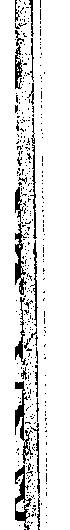
\includegraphics[height=60mm]{figures/gelfand-p000004-margin-left-part01-original-r1.png}\hspace{2mm}
\includegraphics[height=60mm]{figures/gelfand-p000004-margin-left-part02-original-r1.png}\hspace{2mm}
\includegraphics[height=60mm]{figures/gelfand-p000004-margin-left-part03-original-r1.png}\hspace{2mm}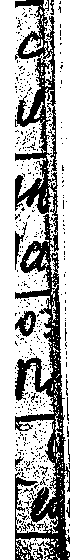
\includegraphics[height=60mm]{figures/gelfand-p000004-margin-left-part04-original-r1.png}}
\expandafter\def\csname evidence-GELFAND-P000005-exponential-rate\endcsname{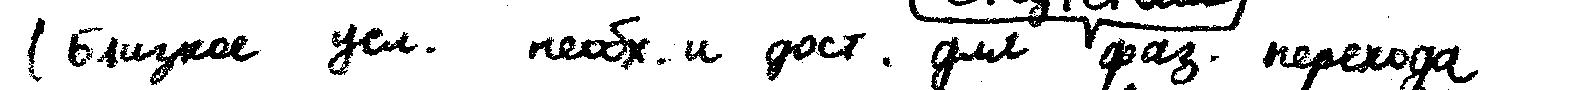
\includegraphics[width=\linewidth]{figures/gelfand-p000005-exponential-rate-part01-original-r1.png}\par\smallskip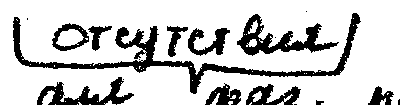
\includegraphics[width=\linewidth]{figures/gelfand-p000005-exponential-rate-part02-original-r1.png}\par\smallskip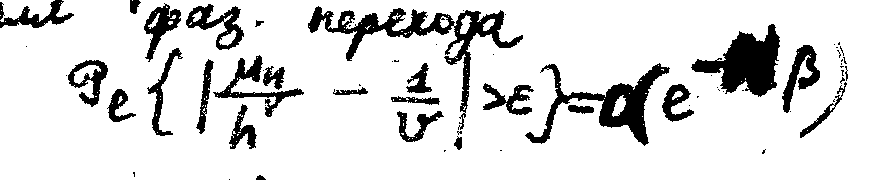
\includegraphics[width=\linewidth]{figures/gelfand-p000005-exponential-rate-part03-original-r2.png}}
\expandafter\def\csname evidence-GELFAND-P000005-complement-label\endcsname{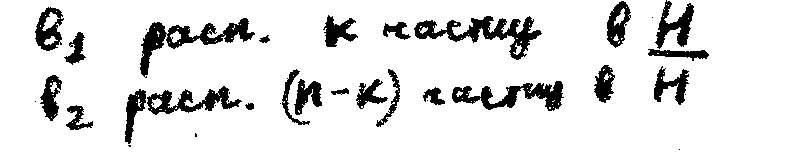
\includegraphics[width=\linewidth]{figures/gelfand-p000005-complement-label-part01-original-r1.png}}
\expandafter\def\csname evidence-GELFAND-P000005-boundary-exponent\endcsname{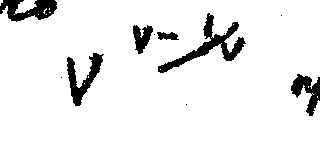
\includegraphics[width=\linewidth]{figures/gelfand-p000005-boundary-exponent-part01-original-r1.png}\par\smallskip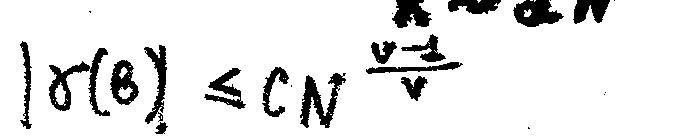
\includegraphics[width=\linewidth]{figures/gelfand-p000005-boundary-exponent-part02-original-r1.png}}
\expandafter\def\csname evidence-GELFAND-P000005-theta-factor\endcsname{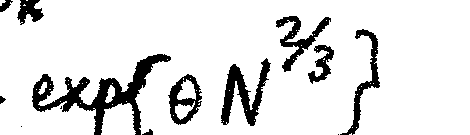
\includegraphics[width=\linewidth]{figures/gelfand-p000005-theta-factor-part01-original-r1.png}\par\smallskip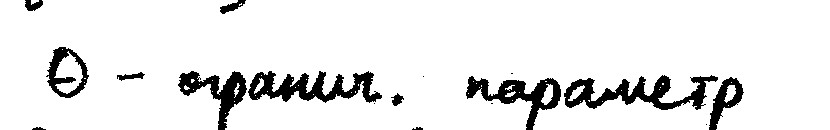
\includegraphics[width=\linewidth]{figures/gelfand-p000005-theta-factor-part02-original-r1.png}\par\smallskip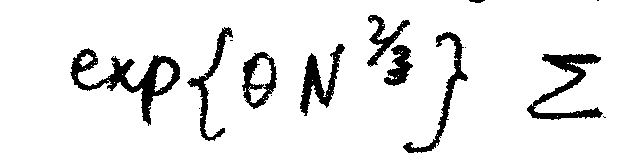
\includegraphics[width=\linewidth]{figures/gelfand-p000005-theta-factor-part03-original-r1.png}}
\expandafter\def\csname evidence-GELFAND-P000005-physical-meaning-heading\endcsname{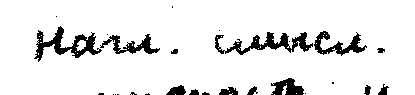
\includegraphics[width=\linewidth]{figures/gelfand-p000005-physical-meaning-heading-part01-original-r1.png}}
\expandafter\def\csname evidence-GELFAND-P000004-diagram-pressure-plateau\endcsname{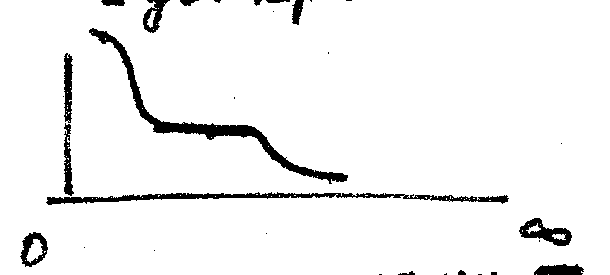
\includegraphics[width=\linewidth]{figures/gelfand-p000004-diagram-pressure-plateau-original-r1.png}}
\newcommand{\PhaseWords}{points of phase\\transition}
\begin{document}
{\large\bfseries Gelfand seminar — chapter 1}\par
{\small Opening of the reader. Source frames 1–5. Text and formulas are typed; original details accompany every uncertain reading. Working excerpt; the complete chapter is still in preparation.}\par\medskip
\SourcePage{GELFAND-P000001}{unlabelled}
Monday, $21/\mathrm{IX}$.
Cartesian and Boolean products of groups.

``Hironaka: on resolution of singularities.''
\underline{Gelfand}

$A$ is a ring, $\mathcal{J}$ is a module over $A$.
\Unclear{GELFAND-P000001}{module-letter}{The letter for the module and ideal is rendered as $\mathcal{J}$; $\mathcal{I}$ or $J$ are possible.}

Blow-up --- ?
$M$ is a manifold; $D\subset M$.
[Beneath $D$:] a subset with singularities.

$M_0^H$ is the blow-up. Blowing-up.
The inverse image of $D$ is $D'$, a manifold of dimension $n-1$.
$D_0$ is $(n-1)$-dimensional.
\SourceFigure{GELFAND-P000001}{diagram-blowup}{Three enclosed drawings: at left a region with $D$; at upper right a region with $D'$ and the label $M_0^H$; at lower right a region and the label $M'_0$. The upper arrow points left; the lower oblique arrow also points left, with the label ``continuous map'' [source abbreviation: непр. отобр.]. The precise inner curves, labels and the connection of the lower region to the upper one require comparison with the scan.}
\Unclear{GELFAND-P000001}{blowup-notation}{The upper index on $M_0$ resembles $H$; the lower region's label resembles $M'_0$.}

The construction is Grothendieck's.
$A$ is a ring, $\mathcal{J}$ is a module.
\underline{Example.} $A$ is a ring of functions;
$\mathcal{J}$ is the ideal of functions taking the value $0$ on $D$.

One obtains a sheaf of rings and a sheaf of modules.
$A$ is a ring, $\mathcal{J}$ is an ideal.
Construct $X$, $O_X$ a sheaf of rings,
$\mathcal{J}_X$ a sheaf of ideals, so that
\begin{gather*}
 (A,\mathcal{J})\ \longleftarrow\ (X,O_X,\mathcal{J}_X).
\end{gather*}
[Beneath the arrow:] linear map.

$(A,\mathcal{J})$ is a sheaf generated by $1$ ideal.

$\mathcal{J}_X$ is invertible, i.e. an ideal of the ring:
$\exists f\in\mathcal{J}_X$ such that $O_Xf=\mathcal{J}_X$.
[Above the formula, an arrow to $\exists$:] generator.

(The ideal is principal if $\mathcal{J}$ is an ideal.)
Then the zero variety is $1$ equation.

$A$ is a ring, $\mathcal{J}$ is an ideal.
\underline{Typical example:} $R^2$, the ideal $=0$ at the origin.
\Unclear{GELFAND-P000001}{origin-example}{The next line: ``Gluing a projective line into $0$'' [source: Вклеив. в $0$ проект. прямой]; the beginning may read ``Оклеив.''.}

$A$, $\mathcal{J}$ are modules.
\begin{gather*}
 \mathcal{J}\otimes_A\mathcal{J},\qquad
 \mathcal{J}\otimes_A\mathcal{J}\otimes_A\mathcal{J},\ldots
\end{gather*}
[Above the groups of tensor products:] symmetric; symmetric.

Consider formal sums
\begin{gather*}
 \sum_{k=0}^{N}a_kz^k.
\end{gather*}
Add and multiply.
$x\otimes y=y\otimes x$.
\begin{gather*}
 a_0\in A,\qquad a_1\in\mathcal{J},\qquad
 a_2\in\mathcal{J}\otimes_A\mathcal{J}\quad\text{—}
\end{gather*}

\SourcePage{GELFAND-P000002}{unlabelled}
The ring of these sums is $S_A(\mathcal{J})$.
Consider homogeneous ideals
[inserted above the line:] (graded).
(Together with a polynomial it contains all its homogeneous components.)

Consider all homogeneous prime ideals in $S_A(\mathcal{J})$.
Выбр. [source abbreviation] ideals which contain all polynomials, starting with degree $1$.
\Unclear{GELFAND-P000002}{ideal-selection}{The end of the line after ``contain all'' is better read as ``polynomials, starting with degree $1$''; the middle strokes of the abbreviation ``нач.'' remain indistinct.}

The collection of ideals is $X$. (The Zariski topology.)
$O_X$, $\mathcal{J}_X$.
If $U$ is an open set, then $O_U$, $\mathcal{J}_U$.
\Unclear{GELFAND-P000002}{open-set-notation}{After ``then'', the first letter has the same form as $O_X$ above, the second as the ideal letter: $O_U$, $\mathcal{J}_U$; the latter may be $\mathcal{I}_U$.}

$S_A(\mathcal{J})$ is the whole ring.
The ring of fractions, numerators, denominators, not belonging to any of the ideals.
Localize the ring at this set.
Fractions of degree $1$: $\mathcal{J}_U$.
\Unclear{GELFAND-P000002}{fractions-sentence}{In the line about fractions, the abbreviations ``numerator--denominator'' and whether ``not belonging'' applies only to the denominator are unclear. No words are supplied from the meaning.}
[At right, two downward arrows:] Grothendieck --- blow up ideally.
\Unclear{GELFAND-P000002}{margin-grothendieck}{The right-hand note reads ``Grothendieck --- blow up ideally''; the last word may be ``идеально'' [ideally] or ``идеалы'' [ideals].}

$A$ is the ring of polynomials in $2$ variables.
$\mathcal{J}$ is the ideal of polynomials with $P(0,0)=0$.
\begin{gather*}
 A=\{P(x,y)\},\qquad
 \mathcal{J}=P(x,y)=a_1x+b_1y+\cdots .
\end{gather*}
\begin{gather*}
 \mathcal{J}\otimes_A\mathcal{J}\ \longleftrightarrow
 \{a_2x^2+2b_2xy+cy^2+\cdots\}.
\end{gather*}
\Unclear{GELFAND-P000002}{quadratic-coefficients}{The coefficients in the quadratic polynomial read $a_2$, $2b_2$, $c$; the index on $c$ and the shape of the thick two-headed arrow are uncertain.}

Because of the interchange, one obtains the same as the square of the ideal.
Then --- the ideal of polynomials equal to $0$ at this point.
What will it blow up into? ?

\begin{gather*}
 \sum P_k(x,y)z^k,\qquad P_k(x,y)=ax^k+\cdots .
\end{gather*}
[At right:] Graded $\Sigma$ of tensor products.
\begin{gather*}
 A=\{P_0(x,y)\}\longrightarrow S_A(\mathcal{J}),\qquad
 P_0(x,y)\sim P_0(x,y).
\end{gather*}
The set of prime ideals obtained from the ideal $P(0,0)=0$.
\begin{gather*}
 S_A\sim\sum P_kz^k,\qquad P_k\in\mathcal{J}^k,\qquad
 K\sim\sum P_kz^k.
\end{gather*}
It suffices to find the max. ideals of the quotient ring ---
(to find the ideals containing the given one).
\begin{gather*}
 S_A/K\ \longleftrightarrow\ a_0+(a_1x-b_1y)z+\cdots .
\end{gather*}
\Unclear{GELFAND-P000002}{last-sign}{In the last formula a minus is visible before $b_1y$, although the next scan has a plus. The visible minus is retained; the direction of the thick arrow is also uncertain.}

\SourcePage{GELFAND-P000003}{2}
All homogeneous max. ideals in it will be the points of the extension.
There is no constant term (then also $1$).
\begin{gather*}
 (a_1x+b_1y)z.
\end{gather*}
Only $1$ linear combination of $x$ and $y$.
(Not $2$, since then all.)

The ideals determine directions in the plane
(замк. [source abbreviation] with all possible directions --- the $\sigma$-process).
\Unclear{GELFAND-P000003}{directions}{The abbreviations in parentheses read ``замк. всеми возм. напр.''; neither the first word nor the meaning of the sign $\sigma$ is asserted.}
\Needspace{48mm}\underline{Problem.} In the space
[cancelled:] \Unclear{GELFAND-P000003}{cross-cancellation}{The cancelled word before the drawing is illegible.}
\par\smallskip\noindent\begin{minipage}{\linewidth}\begin{minipage}[t]{.47\linewidth}\centering\vspace{0pt}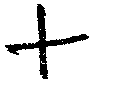
\includegraphics[width=30mm]{figures/gelfand-p000003-cross-diagram-original-r1.png}\par{\scriptsize Original diagram}\end{minipage}\hfill\begin{minipage}[t]{.49\linewidth}\centering\vspace{0pt}\begin{tikzpicture}[scale=0.5]
 \draw (-0.8,0)--(0.8,0);
 \draw (0,-0.7)--(0,0.8);
\end{tikzpicture}\par{\scriptsize Typeset recreation}\end{minipage}\end{minipage}\par\smallskip
What results from gluing it in?
\begin{gather*}
 z=0,\qquad xy=0,\qquad \mathcal{J}=(z,xy).
\end{gather*}
[A line is drawn beneath the system.]

\underline{Dobrushin.}
[Cancelled before ``Find'':] \Unclear{GELFAND-P000003}{ising-cancellation}{The cancelled beginning of the line cannot be read confidently.}
Find an example of a gas in which phase transitions occur.
A cube of the integer lattice.
$\ell$ is the length. $V_\ell=\ell^\nu$.
$N$ points, $N<V_\ell$.
They can occupy positions on the lattice
$\theta=(x_1,\ldots,x_N)$.
\Unclear{GELFAND-P000003}{configuration-letter}{The configuration sign is rendered as $\theta$; the handwritten sign also resembles $b$ or Cyrillic ``в''.}

The Ising model.
[Before the formula, a densely cancelled sign:]
\Unclear{GELFAND-P000003}{energy-cancellation}{The separate cancelled sign before $U(\theta)$ is illegible.}
\begin{gather*}
 U(\theta)=-\frac12\sum_{i\ne j}u(x_i,x_j),\qquad
 u=\begin{cases}
 0&\text{in the other cases},\\
 1;&\rho(x_i,x_j)=1.
 \end{cases}
\end{gather*}
$u(\theta)$ is the number of pairs of neighboring points.
\Unclear{GELFAND-P000003}{energy-case}{In the condition for the second branch a sign resembling $\rho$ is visible; the semicolon after $1$ is retained. In the caption below, the first letter resembles lowercase $u$ rather than $U$.}

The basic axiom is the Gibbs distribution.
\begin{gather*}
 \mathsf{P}(B)=
 \frac{\displaystyle\sum_{\theta\in B}\exp\{-U(\theta)/T\}}
 {Z(V_\ell,N)},\qquad T>0\text{ --- temperature.}
\end{gather*}
[Beneath the denominator:] normalizing factor.
\begin{gather*}
 Z(\ell,N)=\sum_{\theta\in\mathcal{B}}\exp\{-U(\theta)/T\}.
\end{gather*}
\Unclear{GELFAND-P000003}{partition-domain}{The denominator in the first formula reads $Z(V_\ell,N)$, the next line $Z(\ell,N)$; the set sign beneath the sum resembles $\mathcal{B}$. The notation is not adjusted for consistency.}

The molecules attract one another.
([Two filled signs with arrows:] neighbors $>$ their probability.)
\Unclear{GELFAND-P000003}{attraction-note}{In parentheses after ``The molecules attract'', there are filled signs and arrows; the reading ``neighbors $>$ their probability'' is uncertain.}
$B\subset\mathcal{B}$ is a collection of configurations.
\begin{gather*}
 p(\theta)=\frac{\exp\{-U(\theta)/T\}}{Z(\ell,N)}.
\end{gather*}
Take the limit $\ell\to\infty$; the cube expands to $\infty$.
$N_\ell$ depends on $\ell$.
[A cancelled sign before the fraction:]
\Unclear{GELFAND-P000003}{density-cancellation}{The cancelled sign before $V_\ell/N_\ell$ is illegible.}
\begin{gather*}
 \frac{V_\ell}{N_\ell}=v=\mathrm{const}.
\end{gather*}
The lattice grows.
One can show that
\begin{gather*}
 \frac1{N_\ell}\log Z(\ell,N_\ell)\longrightarrow f(v,T).
\end{gather*}

\SourcePage{GELFAND-P000004}{unlabelled}
\begin{gather*}
 p(v,T)=T\frac{\partial f}{\partial v}\qquad\text{by definition.}
\end{gather*}
\Unclear{GELFAND-P000004}{pressure-letter}{The heavily written first argument of $p$ resembles $v$; no minus is visible before the derivative, and none is supplied.}

Phase transition.
As for $f$: it is a monotone, convex function of $v$.
Therefore $p>0$, and $p$ is a monotone function of $v$.
Phase transition: $p(v,T)$ has a flat segment.
\SourceFigure{GELFAND-P000004}{diagram-phase-point}{In the upper right-hand field is a bent, S-like curve with an almost horizontal middle segment and an arrow toward it; the caption reads ``points of phase transition'' [source abbreviation: точки фаз. перехода]. Precise axes and points in the original drawing are not identified confidently.\par\smallskip\centering\resizebox{.93\linewidth}{!}{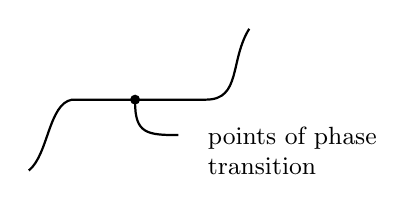
\begin{tikzpicture}[x=1cm,y=1cm]
\draw[thick] (0,0)..controls(.25,.2)and(.25,.85)..(.55,.9)--(2.25,.9)..controls(2.7,.9)and(2.55,1.4)..(2.8,1.8);
\fill(1.35,.9)circle(1.8pt);
\draw[thick](1.35,.87)..controls(1.35,.47)and(1.5,.45)..(1.9,.45);
\node[anchor=west,align=left,font=\small]at(2.15,.25){\PhaseWords};
\end{tikzpicture}}\par{\scriptsize Typeset sketch; limitations are recorded in the note.}\par}
There is a physical hypothesis: $1$ transition segment.

\SourceFigure{GELFAND-P000004}{diagram-cancelled-graph}{At left is a graph with vertical and horizontal axes, $0$ and $\infty$ by the horizontal axis. Several curves and straight lines are heavily crossed out; the precise cancelled curve and the vertical label need comparison.\par\smallskip\centering\resizebox{.93\linewidth}{!}{\begin{tikzpicture}[x=1cm,y=1cm]
\draw[thick](0,1.75)--(0,0)--(3.6,0);
\node[below]at(0,-.05){$0$};\node[below]at(3.6,-.05){$\infty$};
\end{tikzpicture}}\par{\scriptsize Partial recreation: secure axes only; cancelled curves remain unresolved.}\par}
\SourceFigure{GELFAND-P000004}{diagram-pressure-plateau}{Neighboring drawing at right: a clean descending curve with a flat segment. This is a separate graph, not a reconstruction of the cancelled drawing at left.\par\smallskip\centering\resizebox{.9\linewidth}{!}{\begin{tikzpicture}[scale=0.7]
 \draw (0,0)--(4.6,0);
 \draw (0,0)--(0,2.3);
 \draw (0.2,2.5).. controls (0.9,2.4) and (0.5,1.25)..(1.2,1.15)
 --(2.4,1.15).. controls (2.9,1.05) and (2.7,0.45)..(4,0.35);
 \node at (-0.1,-0.4) {$0$};
 \node at (4.6,-0.4) {$\infty$};
\end{tikzpicture}}\par{\scriptsize Existing typeset recreation.}}
A flat segment occurs for sufficiently small $T$ ($<T_{\text{crit}}$).

It admits an explicit solution for $n=1$.
$Z$ and $f(v,T)$ are calculated.
There are no phase transitions, which is considered physically natural.

\underline{$n=2$.} \underline{Onsager.}
$f(v,T)$ is calculated for particular $v$ and $T$.
A discontinuity of the derivative corresponds to phase transitions.
\SourceFigure{GELFAND-P000004}{diagram-onsager}{A graph with the $T$ axis upward, the $v$ axis to the right, and the label $1/2$ beneath a vertical through the vertex. The curve rises from the left to the vertex and descends to the right; the vertical line passes through the vertex, with a short wavy segment to its right. The precise geometry and the meaning of the wavy branch have not been established.\par\smallskip\centering\resizebox{.93\linewidth}{!}{\begin{tikzpicture}[x=1cm,y=1cm]
\draw(0,0)--(4.6,0);\draw(0,0)--(0,2.3);
\node[left]at(0,2.3){$T$};\node[below]at(4.6,0){$v$};
\draw(2.2,-.05)--(2.2,2.65);\node[below]at(2.2,-.12){$1/2$};
\draw[thick](.7,-.02)..controls(1.25,.35)and(1.85,.95)..(2.2,1.35)..controls(2.4,1.1)and(3.05,.55)..(3.45,.18);
\draw(1.05,.18)..controls(1.5,.54)and(1.9,1)..(2.17,1.35);
\fill(2.2,1.35)circle(1.5pt);
\draw[thick](2.32,1.4)..controls(2.5,1.62)and(2.63,1.33)..(2.78,1.42)..controls(2.86,1.47)and(2.98,1.56)..(3.03,1.61);
\end{tikzpicture}}\par{\scriptsize Typeset sketch; limitations are recorded in the note.}\par}

Kac, Helfand.
Exact, in explicit form, for some cases [source endings: точн. в яв. виду для нек-рых случаях].
\Unclear{GELFAND-P000004}{kac-helfand-note}{After another enlargement, the line reads ``точн. в яв. виду для нек-рых случаях''; the endings may instead be ``виде'' and ``случаев''. The ungrammatical reading is not corrected automatically.}

\SourceFigure{GELFAND-P000004}{diagram-subcube}{A large square with a smaller outlined region inside; $H$ at its center and $h$ above the smaller region. The small contour is partly square and partly rounded; its precise boundary has not been reconstructed.\par\smallskip\centering\resizebox{.93\linewidth}{!}{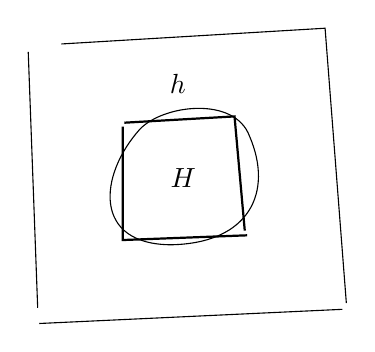
\begin{tikzpicture}[x=1cm,y=1cm]
\draw(.3,3.45)--(3.65,3.65)--(3.92,.16);\draw(3.87,.08)--(.02,-.1);\draw(0,.1)--(-.12,3.35);
\draw[thick](1.1,2.45)--(2.5,2.53)--(2.63,1.08);\draw[thick](2.66,1.02)--(1.08,.96)--(1.08,2.4);
\draw(1.3,2.37)..controls(1.6,2.68)and(2.5,2.79)..(2.69,2.28)..controls(3,1.56)and(2.68,.92)..(1.7,.9)..controls(.7,.9)and(.77,1.78)..(1.3,2.37);
\node at(1.85,1.75){$H$};\node at(1.78,2.94){$h$};
\end{tikzpicture}}\par{\scriptsize Typeset sketch; limitations are recorded in the note.}\par}
\begin{gather*}
 \frac{\mu_H}{h^\nu}.
\end{gather*}
$\mu_H$ is the number of particles in $H$ --- a subcube.
$\nu$ is the dimension.
\begin{gather*}
 \frac{\mu_H}{h^\nu}=\frac1v\qquad\text{as in the whole space.}
\end{gather*}
\underline{Law of large numbers.}
\begin{gather*}
 \mathsf{P}\left\{\frac{\mu_H}{h^\nu}-\frac1v\,\middle|\,>\varepsilon\right\}
 \longrightarrow0.
\end{gather*}
\Unclear{GELFAND-P000004}{probability-bar}{In the probability formula the right vertical bar before $>\varepsilon$ is visible; a left bar before the fraction has not been read confidently. No matching bar is silently supplied.}
\begin{gather*}
 \ell\to\infty,\qquad H\to\infty,\qquad
 d<\frac h\ell<1-d,\qquad d>0.
\end{gather*}
\Unclear{GELFAND-P000004}{bottom-mark}{At the lower right edge a small sign resembles ``2'' or a broken-off letter; it has not been adopted as a page number.}
\Incomplete{GELFAND-P000004}{margin-left}{Along the extreme left edge is a narrow strip of neighboring handwritten text, cropped to isolated endings and strokes; no connected text can be read.}


\SourcePage{GELFAND-P000005}{3}
If this does \underline{not} hold, a phase transition takes place.
\Unclear{GELFAND-P000005}{physical-meaning-heading}{Нагл. [candidate abbreviation; the middle strokes are not fully distinguishable]} meaning. $2$ phases coexist; the particles are distributed unevenly ---
--- liquid and gas.
[Above the line:] (law of large numbers).
[Inserted above ``phase transition'', with a bracket:] absence.
(A closely related condition is necessary and sufficient for a phase transition
\begin{gather*}
 \mathsf{P}_\ell\left\{\left|\frac{\mu_H}{h^\nu}-\frac1v\right|>\varepsilon\right\}
 =O(e^{-N\beta}).
\end{gather*}
\Unclear{GELFAND-P000005}{exponential-rate}{The exponent of $e$ contains a heavily written sign before $\beta$; the candidate is $-N\beta$, but $N$ is obscured by overlapping strokes. The parenthesis opened before ``A closely related'' is not clearly closed in the scan.}
[At right:] $N$ is the number of particles.

Calculate the probability that
\begin{gather*}
 \mathsf{P}\{\mu_H=k\}=Z^{-1}
 \sum_{\theta\in\mathcal{B}_k}\exp\{-U(\theta)/T\}.
\end{gather*}
Over configurations in which $H$ contains $k$ particles.
$\theta$ is a configuration of $N$ particles.
$\theta\in\mathcal{B}_k$.
Then $\theta=(\theta_1,\theta_2)$.
$\theta_1$ is a configuration of $k$ particles in $H$.
$\theta_2$ is a configuration of $(N-k)$ particles in $\overline H$.
\Unclear{GELFAND-P000005}{complement-label}{The upper bar on $H$ in the line about $\theta_2$ is not completely distinct; the candidate is $\overline H$.}
\begin{gather*}
 U(\theta)=U(\theta_1)+U(\theta_2)+\gamma(\theta).
\end{gather*}
$U(\theta_1)$ is the interaction inside.
$U(\theta_2)$: neighbors outside.
$\gamma(\theta)$ is the interaction across the surface.
$\gamma(\theta)$ can be neglected asymptotically.
(Across the boundary: of the order of the number of boundary points)
$V^{\nu-1/\nu}$ as $N\to\infty$.
$k\sim dN$.
\Unclear{GELFAND-P000005}{boundary-exponent}{The exponent on $V$ looks like $\nu-1/\nu$, without a confidently distinguishable common numerator. It has not been changed automatically to $(\nu-1)/\nu$.}
\begin{gather*}
 |\gamma(\theta)|\le CN^{\frac{\nu-1}{\nu}}.
\end{gather*}
\begin{align*}
 \sum\exp\{-U(\theta)/T\}
 &=\sum_{\theta\in\mathcal{B}_k}\exp\{-U(\theta_1)/T\}
 \exp\{-U(\theta_2)/T\}\\
 &\qquad\times
 \exp\{\theta N^{2/3}\}
 =
\end{align*}
\Unclear{GELFAND-P000005}{theta-factor}{The letter before $N^{2/3}$ resembles $\theta$ or $\Theta$; below, the same letter is glossed as ``bounded parameter''. It may differ from the configuration sign.}
$\theta$ is a bounded parameter.
\begin{gather*}
 =\exp\{\theta N^{2/3}\}
 \sum_{\theta_1}\exp\{-U(\theta_1)/T\}
 \sum_{\theta_2}\exp\{-U(\theta_2)/T\}.
\end{gather*}
[Beneath the first sum:] configurations.

\clearpage\section*{Full reading notes}
\subsection*{GELFAND-0001-U001}
\EvidenceBlock{GELFAND-P000001}{module-letter}{After “A is a ring” is a handwritten letter with a fork at the top and a lower hook; it recurs for the module and the ideal.}{Observation.}
\par\smallskip\noindent\textbf{Candidates: } \(\mathcal{J}\); \(\mathcal{I}\); J\par
\par\smallskip\noindent\textbf{Historical note: } A calligraphic J was used in the text as a graphical candidate; the notation was not identified from its mathematical meaning.\par
\par\smallskip\noindent\textbf{Fresh source comparison: } The same fork and lower hook are visible in three separate occurrences at 5×/10×. This supports a consistent graphical transcription but does not distinguish every possible conventional I/J letterform.\par
\subsection*{GELFAND-0001-U002}
\EvidenceBlock{GELFAND-P000001}{diagram-blowup}{In the upper half are three rounded contours with inner curves and two leftward arrows; D, D-prime, M and indices occur above and beside them.}{Observation.}
\par\smallskip\noindent\textbf{Candidates: } None proposed.\par
\par\smallskip\noindent\textbf{Historical note: } Uncertain inner curves and joins were not redrawn. The description and the source-figure entry retain a locator for comparison.\par
\par\smallskip\noindent\textbf{Fresh source comparison: } The complete diagram crop is now displayed at its typed description. Both leftward arrowheads are visible. A separate curved stroke rises from the lower contour toward the area beside D; its exact attachment to the upper contour is not asserted.\par
\subsection*{GELFAND-0001-U003}
\EvidenceBlock{GELFAND-P000001}{blowup-notation}{The upper index on \(M_0\) resembles H; over \(M_0\) at the lower region is a short stroke.}{Observation.}
\par\smallskip\noindent\textbf{Candidates: } \(M_0^H\); \(M'_0\); \(M_0^N\); \(M'_0\)\par
\par\smallskip\noindent\textbf{Historical note: } The indices and prime need comparison with the original.\par
\par\smallskip\noindent\textbf{Fresh source comparison: } Separate close crops show the dark upper index and the lower prime at the reading itself. The lower prime is distinct; the dark upper sign still does not justify excluding N in favor of H.\par
\subsection*{GELFAND-0001-U006}
\EvidenceBlock{GELFAND-P000001}{origin-example}{To the right of the \(R^2\) example the line begins with a joined group of letters and ends “into 0, a projective line”.}{Observation.}
\par\smallskip\noindent\textbf{Candidates: } Вклеив. в 0 проект. прямой [Gluing a projective line into 0]; Оклеив. в 0 проект. прямой [alternative initial abbreviation]\par
\par\smallskip\noindent\textbf{Historical note: } The phrase is given inside the uncertain-reading entry, without choosing from the mathematical meaning of a blow-up.\par
\par\smallskip\noindent\textbf{Fresh source comparison: } The wider context and 5×/10× details strongly favor the initial В and the abbreviation Вклеив. The historical alternative remains visible; the source wording is not replaced by a standard construction of a blow-up.\par

\subsection*{GELFAND-0001-U007}
\EvidenceBlock{GELFAND-P000002}{ideal-selection}{A rereading of the enlarged original fragment favors “polynomials, starting with degree 1”; the middle strokes of the abbreviation нач. are still not fully distinguishable.}{Observation.}
\par\smallskip\noindent\textbf{Candidates: } мн., нач. с 1-й степени [polynomials, starting with degree 1]; мн., к-ст. с 1-й степенью [alternative abbreviation; expansion uncertain]\par
\par\smallskip\noindent\textbf{Historical note: } The first candidate was selected from the shape of the original line; it was not replaced by the standard definition of Proj.\par
\par\smallskip\noindent\textbf{Fresh source comparison: } The line ending is visible in the wider crop and separate 5×/10× details. Its first abbreviation Выбр. is visible too, but its expansion could express selecting or discarding. The English text retains that abbreviation rather than deciding the operation from the construction. The strokes favor нач. at the end; the historical alternative remains recorded.\par

\subsection*{GELFAND-0001-U008}
\EvidenceBlock{GELFAND-P000002}{open-set-notation}{In a separate rereading, the first letter after “then” matches the shape of \(O_X\) above; the second matches the ideal letter with a lower hook.}{Observation.}
\par\smallskip\noindent\textbf{Candidates: } \(O_U,J_U\); \(O_U,I_U\)\par
\par\smallskip\noindent\textbf{Historical note: } The initial reading of the first letter as J was corrected from the scan. The possible I/J distinction in the second letter remains, independently of the standard sheaf construction.\par
\par\smallskip\noindent\textbf{Fresh source comparison: } The corrected context now includes the whole lower subscripts. The rounded first sign and forked, hooked second sign match the earlier pair. These shapes support O followed by the ideal letter, without deciding every conventional I/J distinction. Separate 5×/10× details were inspected.\par

\subsection*{GELFAND-0001-U009}
\EvidenceBlock{GELFAND-P000002}{fractions-sentence}{After “ring of fractions” one can see “numer., denom., not belonging to any of the ideals”, but the abbreviation boundaries and the scope of the last phrase are unclear.}{Observation.}
\par\smallskip\noindent\textbf{Candidates: } числ., знамен., не прин. ни одному из идеалов [numer., denom., not belonging to any of the ideals]; числ.; знамен. не прин. ни одному из идеалов [numer.; denom. not belonging to any of the ideals]\par
\par\smallskip\noindent\textbf{Historical note: } The punctuation was not corrected from the definition of localization.\par
\par\smallskip\noindent\textbf{Fresh source comparison: } Four overlapping source parts retain the line ending числ., the following знамен., and the phrase about the ideals. The abbreviations are visible at 5×/10×; their punctuation does not establish which nouns the restriction modifies. No missing qualifier is supplied.\par

\subsection*{GELFAND-0001-U010}
\EvidenceBlock{GELFAND-P000002}{margin-grothendieck}{The right-hand note beside two vertical arrows reads “Grothendieck — blow up …”; the final word is written continuously.}{Observation.}
\par\smallskip\noindent\textbf{Candidates: } идеально [ideally]; идеалы [ideals]\par
\par\smallskip\noindent\textbf{Historical note: } The final word is not asserted.\par
\par\smallskip\noindent\textbf{Fresh source comparison: } The wider crop includes both downward arrows and the full note. The joined final strokes favor идеально, but do not securely exclude идеалы. The literal candidate “blow up ideally” is retained with the alternative; the wording is not regularized into a definition.\par

\subsection*{GELFAND-0001-U011}
\EvidenceBlock{GELFAND-P000002}{quadratic-coefficients}{After J tensor J is a thick two-sided mark and a quadratic polynomial; the coefficients resemble \(a_2\), \(2b_2\), c.}{Observation.}
\par\smallskip\noindent\textbf{Candidates: } \(a_2x^2+2b_2xy+cy^2+\cdots\); \(a_2x^2+2b_2xy+c_2y^2+\cdots\)\par
\par\smallskip\noindent\textbf{Historical note: } The index on the final coefficient and the direction of the thick mark are uncertain.\par
\par\smallskip\noindent\textbf{Fresh source comparison: } The complete context and separate details show \(a_2\) and \(2b_2\). A small upper stroke is visible near the c-shaped coefficient; it is not a secure lower index 2. The thick connecting mark is retained as an uncertain graphical candidate, without inferring an isomorphism.\par

\subsection*{GELFAND-0001-U012}
\EvidenceBlock{GELFAND-P000002}{last-sign}{At the lower edge is \(a_0+(a_1x-b_1y)z+\cdots\); the horizontal sign before \(b_1y\) looks like a minus.}{Observation.}
\par\smallskip\noindent\textbf{Candidates: } \(a_0+(a_1x-b_1y)z+\cdots\); \(a_0+(a_1x+b_1y)z+\cdots\)\par
\par\smallskip\noindent\textbf{Historical note: } The visible minus is retained in the body; the next scan has a plus. The arrow at left is written heavily.\par
\par\smallskip\noindent\textbf{Fresh source comparison: } The enlarged sign is a horizontal minus; no vertical crossing stroke is visible. The next source page has a plus. Both source readings remain, and the mathematical commentary does not use a change of sign to alter either transcription. The heavy arrow still has uncertain direction.\par

\subsection*{GELFAND-0001-U013}
\EvidenceBlock{GELFAND-P000003}{directions}{In parentheses after “plane” is the abbreviation “замк. всеми возм. напр.” and a sign resembling sigma before “process”.}{Observation.}
\par\smallskip\noindent\textbf{Candidates: } замк. всеми возм. напр. — σ-процесс [first abbreviation uncertain; with all possible directions — sigma-process]; зам. всеми возм. напр. — σ-процесс [alternative first abbreviation; with all possible directions — sigma-process]\par
\par\smallskip\noindent\textbf{Historical note: } The abbreviations were not expanded or replaced by a term inferred from the meaning.\par
\par\smallskip\noindent\textbf{Fresh source comparison: } The initial abbreviation and the sigma-like sign have been inspected at 5×/10×. The final short stroke of the first abbreviation is still not secure. The translation expands the readily legible neighboring abbreviations, but keeps замк. itself visibly unexpanded.\par

\subsection*{GELFAND-0001-U014}
\EvidenceBlock{GELFAND-P000003}{cross-cancellation}{Between “In the space” and the cross is a heavily cancelled short group of letters.}{Observation.}
\par\smallskip\noindent\textbf{Candidates: } None proposed.\par
\par\smallskip\noindent\textbf{Historical note: } The cancellation itself is marked; the underlying text cannot be read confidently.\par
\par\smallskip\noindent\textbf{Fresh source comparison: } The opaque horizontal cancellation remains unreadable even at 10×. The separate original cross is also shown beside the existing two-stroke native recreation. Its thick ends do not establish intentional arrowheads; the recreation retains two crossing, unarrowed strokes.\par

\subsection*{GELFAND-0001-U016}
\EvidenceBlock{GELFAND-P000003}{ising-cancellation}{Under the name Dobrushin, before “Find”, a group of letters is completely crossed out.}{Observation.}
\par\smallskip\noindent\textbf{Candidates: } None proposed.\par
\par\smallskip\noindent\textbf{Historical note: } The visible cancellation is preserved; the original word was not reconstructed.\par
\par\smallskip\noindent\textbf{Fresh source comparison: } The wider context identifies the position before “Find”; the 5×/10× details show multiple dense crossing strokes. They do not support a complete word, so no candidate is invented.\par

\subsection*{GELFAND-0001-U017}
\EvidenceBlock{GELFAND-P000003}{configuration-letter}{Before \((x_1,\ldots,x_N)\), and later in the formulas, is a sign with a rounded lower part and a dark upper stroke.}{Observation.}
\par\smallskip\noindent\textbf{Candidates: } \(\theta\); \(b\); в\par
\par\smallskip\noindent\textbf{Historical note: } The fragment uses theta as a single graphical candidate for this recurring sign.\par
\par\smallskip\noindent\textbf{Fresh source comparison: } The corrected crop includes the entire left-hand sign and its equality. Two separate occurrences were inspected at 5×/10×. The divided loop and thick upper stroke are consistent, but do not securely exclude b or Cyrillic в. The theta transcription remains explicitly provisional.\par

\subsection*{GELFAND-0001-U018}
\EvidenceBlock{GELFAND-P000003}{energy-cancellation}{Between “The Ising model” and \(U(\theta)\) is a separate completely inked-out sign.}{Observation.}
\par\smallskip\noindent\textbf{Candidates: } None proposed.\par
\par\smallskip\noindent\textbf{Historical note: } The cancelled sign was not taken as a mathematical operator.\par
\par\smallskip\noindent\textbf{Fresh source comparison: } The sign remains opaque at 5×/10×; its dark mass and the underlying strokes do not identify an operator or letter. Its location and cancellation are preserved, without assigning it a mathematical role.\par

\subsection*{GELFAND-0001-U019}
\EvidenceBlock{GELFAND-P000003}{energy-case}{In the second branch of u=..., the sign before \((x_i,x_j)=1\) resembles rho; the caption below begins \(u(\theta)\).}{Observation.}
\par\smallskip\noindent\textbf{Candidates: } \(\rho(x_i,x_j)=1\); \(\chi(x_i,x_j)=1\)\par
\par\smallskip\noindent\textbf{Historical note: } A sign resembling a semicolon is visible after the unit value. The small u in the caption was not replaced with U.\par
\par\smallskip\noindent\textbf{Fresh source comparison: } A corrected context contains the complete equality, and a repaired 5×/10× target shows the rho-shaped letter itself. The earlier narrow detail missed that target and is not used as evidence for it. The full lower caption clearly begins with a small u-shaped letter. The branch punctuation and the U/u difference remain diplomatic; their mathematical implications are discussed separately.\par

\subsection*{GELFAND-0001-U020}
\EvidenceBlock{GELFAND-P000003}{partition-domain}{The first normalizing quantity looks like \(Z(V_\ell,N)\); below is \(Z(\ell,N)\). The set under the second sum has the shape of a handwritten B.}{Observation.}
\par\smallskip\noindent\textbf{Candidates: } \(Z(V_\ell,N);\ Z(\ell,N);\ \theta\in B\); \(Z(V_\ell,N);\ Z(\ell,N);\ \theta\in\mathcal B\)\par
\par\smallskip\noindent\textbf{Historical note: } The difference in arguments is preserved. The set symbol was not identified with the event B from its meaning.\par
\par\smallskip\noindent\textbf{Fresh source comparison: } Separate 5×/10× details confirm the visible \(V_\ell\) in the first denominator and ell in the next line. The set under the second sum carries an added upper stroke, supporting a distinct graphical candidate, but ordinary B versus a calligraphic form remains uncertain. The transcription keeps the event and configuration-set candidates distinct.\par

\subsection*{GELFAND-0001-U021}
\EvidenceBlock{GELFAND-P000003}{attraction-note}{After “The molecules attract” are parentheses with inked signs, arrows, and the words “neighbors” and “probab.”.}{Observation.}
\par\smallskip\noindent\textbf{Candidates: } соседи > их вероятн. [neighbors > their probab.]; соседи > его вероятн. [neighbors > its probab.]\par
\par\smallskip\noindent\textbf{Historical note: } The provisional caption was given only as a candidate; the drawing was not converted into a precise assertion.\par
\par\smallskip\noindent\textbf{Fresh source comparison: } The filled marks, arrows and caption are displayed together. At 5×/10× the pronoun looks closer to его than to их, but the elliptical phrase still does not support a complete assertion. The inherited body candidate remains visibly marked as uncertain and both historical alternatives are retained.\par

\subsection*{GELFAND-0001-U022}
\EvidenceBlock{GELFAND-P000003}{density-cancellation}{Before \(V_\ell/N_\ell\) is a heavily cancelled short mark.}{Observation.}
\par\smallskip\noindent\textbf{Candidates: } None proposed.\par
\par\smallskip\noindent\textbf{Historical note: } The original sign was not recovered.\par
\par\smallskip\noindent\textbf{Fresh source comparison: } The cancelled mark remains unreadable in the enlarged details. The wider source fragment includes the fraction and \(v=\mathrm{const}\), so its place is inspectable. The written ratio \(V_\ell/N_\ell\) is retained, rather than silently changed to particle density \(N_\ell/V_\ell\).\par


\subsection*{GELFAND-0001-U024}
\EvidenceBlock{GELFAND-P000004}{pressure-letter}{The first argument of \(p(\cdot,T)\) is heavily written. The fraction contains \(\partial f/\partial v\) and is preceded by T; no minus is visible before the derivative.}{Observation.}
\par\smallskip\noindent\textbf{Candidates: } \(p(v,T)=T\partial f/\partial v\); \(p(\nu,T)=T\partial f/\partial v\)\par
\par\smallskip\noindent\textbf{Historical note: } No thermodynamically expected correction of the sign was substituted.\par
\par\smallskip\noindent\textbf{Fresh source comparison: } The whole frame and 3×/5×/10× details show no minus before T. The first argument remains a heavily written v-like sign; \(\nu\) is not excluded. A separate commentary derives a possible plus under an explicit definition of f; this does not settle the letter or amend the source.\par

\subsection*{GELFAND-0001-U025}
\EvidenceBlock{GELFAND-P000004}{diagram-phase-point}{The upper right drawing has a rising curve with a flat middle, an arrow toward it, and the caption “points of phase transition” [точки фаз. перехода].}{Observation.}
\par\smallskip\noindent\textbf{Candidates: } None proposed.\par
\par\smallskip\noindent\textbf{Historical note: } The precise axes, points, and shape of the transitions are not identified confidently.\par
\par\smallskip\noindent\textbf{Fresh source comparison: } After extending the crop downward, the whole caption “точки фаз. перехода” is visible, in the plural. No axes are visible. The typeset sketch represents the flat middle, point, and curved pointer; it does not assert the precise direction of the heavily inked arrowhead.\par

\subsection*{GELFAND-0001-U026}
\EvidenceBlock{GELFAND-P000004}{diagram-cancelled-graph}{At left are two axes, with 0 and \(\infty\) by the horizontal axis; several heavily overwritten curves and straight lines, and a vertical letter.}{Observation.}
\par\smallskip\noindent\textbf{Candidates: } vertical label \(\varphi\); vertical label f\par
\par\smallskip\noindent\textbf{Historical note: } The crossed-out lines were retained by description; no precise underlying curve was selected.\par
\par\smallskip\noindent\textbf{Fresh source comparison: } Even at 10×, individual connections of the underlying curves cannot be separated from the heavy cancellations. The partial typeset sketch shows only the secure axes, 0 and \(\infty\); the disputed vertical letter remains among the candidates. The neighboring clean graph at right is a different drawing and is shown separately.\par

\subsection*{GELFAND-0001-U028}
\EvidenceBlock{GELFAND-P000004}{diagram-onsager}{Axes T and v; a curve with a vertex, a vertical through the vertex, \(1/2\) below, and a small wavy branch at right.}{Observation.}
\par\smallskip\noindent\textbf{Candidates: } None proposed.\par
\par\smallskip\noindent\textbf{Historical note: } The branches and their connections require the original drawing; an exact redrawing had not been made.\par
\par\smallskip\noindent\textbf{Fresh source comparison: } The left branch has an additional stroke; the vertical passes through the vertex, with \(1/2\) below. A small visible gap separates the short wavy line at right from the vertex. The typeset sketch retains that gap without assigning physical meaning to the line.\par

\subsection*{GELFAND-0001-U029}
\EvidenceBlock{GELFAND-P000004}{kac-helfand-note}{A repeated twofold enlargement of the line beneath Kac, Helfand shows “точн. в яв. виду для нек-рых случаях” [exact, in explicit form, for some cases]; the word endings are not completely clear.}{Observation.}
\par\smallskip\noindent\textbf{Candidates: } точн. в яв. виду для нек-рых случаях [literal source endings]; точн. в яв. виде для нек-рых случаев [alternative endings]\par
\par\smallskip\noindent\textbf{Historical note: } The word случая... [case...] has now been read, replacing the erroneous initial сущ.; neither grammar nor the known result is used to correct the ending silently.\par
\par\smallskip\noindent\textbf{Fresh source comparison: } The wide crop retains the names and the entire line. The 5×/10× details favor виду and случаях. The historical alternatives виде and случаев remain in full; the English body conveys the meaning while separately displaying the nonstandard source endings.\par

\subsection*{GELFAND-0001-U030}
\EvidenceBlock{GELFAND-P000004}{diagram-subcube}{A large square and a smaller outlined region, H at the center and h above; the small contour has overlapping rounded and straight strokes.}{Observation.}
\par\smallskip\noindent\textbf{Candidates: } None proposed.\par
\par\smallskip\noindent\textbf{Historical note: } The source was retained as a drawing, without selecting an exact boundary from the term “subcube”.\par
\par\smallskip\noindent\textbf{Fresh source comparison: } Both straight and rounded strokes of the inner boundary are visible at 5×/10×; h above H is readable. The outer lines have gaps. The typeset sketch retains the overlap and gaps rather than replacing the drawing with a perfect square or circle.\par

\subsection*{GELFAND-0001-U031}
\EvidenceBlock{GELFAND-P000004}{probability-bar}{A vertical bar is visible before \(>\varepsilon\); before the first fraction, a possible left bar merges with the brace.}{Observation.}
\par\smallskip\noindent\textbf{Candidates: } \(\mathsf P\{\mu_H/h^\nu-1/v\mid>\varepsilon\}\to0\); \(\mathsf P\{|\mu_H/h^\nu-1/v|>\varepsilon\}\to0\)\par
\par\smallskip\noindent\textbf{Historical note: } The matching bar was not added silently; the visible candidate was left in the body.\par
\par\smallskip\noindent\textbf{Fresh source comparison: } The right vertical stroke is separate from \(>\varepsilon\). An independent left absolute-value bar beside the opening brace cannot be established even at 10×. The next frame clearly has paired bars, but that comparison does not change this frame’s notation.\par

\subsection*{GELFAND-0001-U032}
\EvidenceBlock{GELFAND-P000004}{bottom-mark}{At the lower right edge, a small isolated sign resembles 2 or a fragment of a letter.}{Observation.}
\par\smallskip\noindent\textbf{Candidates: } 2; fragment of a letter\par
\par\smallskip\noindent\textbf{Historical note: } No confident page number was assigned.\par
\par\smallskip\noindent\textbf{Fresh source comparison: } At 5×/10×, only a short hook and fragmentary edge strokes remain. The digit 2 and a fragment of a letter remain candidates; no number is assigned.\par

\subsection*{GELFAND-0001-U033}
\EvidenceBlock{GELFAND-P000004}{margin-left}{At the extreme left edge of the frame, a narrow strip of neighboring text is cut off to isolated endings and strokes; a separate crop at native pixel resolution was checked.}{Observation.}
\par\smallskip\noindent\textbf{Candidates: } None proposed.\par
\par\smallskip\noindent\textbf{Historical note: } Connected text is unavailable in this frame; the page has unreadable status because of this portion. The main writing surface has been read and transcribed.\par
\par\smallskip\noindent\textbf{Fresh source comparison: } Four overlapping source strips retain the entire available left edge. It is already clipped in the whole original frame; further magnification cannot restore the missing portions of letters. No independently readable words were established.\par

\subsection*{GELFAND-0001-U034}
\EvidenceBlock{GELFAND-P000005}{exponential-rate}{In \(O(e^{\cdots\beta})\), the sign between the minus and \(\beta\) is heavily obscured; before the preceding phrase is an opening round parenthesis without a clearly visible closing parenthesis.}{Observation.}
\par\smallskip\noindent\textbf{Candidates: } \(O(e^{-N\beta})\); \(O(e^{-\ell\beta})\)\par
\par\smallskip\noindent\textbf{Historical note: } The obscured sign was not declared settled, and a missing parenthesis was not added to the source text.\par
\par\smallskip\noindent\textbf{Fresh source comparison: } The corrected crop includes the tops of all overlapping strokes in the exponent. The minus and \(\beta\) are visible; the intervening sign cannot reliably be distinguished as N or \(\ell\) at 10×. Separate crops show the insertion “absence” and the opening parenthesis. The insertion is retained explicitly, and the parenthesis is not closed editorially.\par

\subsection*{GELFAND-0001-U035}
\EvidenceBlock{GELFAND-P000005}{complement-label}{In the line about \(\theta_2\) and \(N-k\) particles, a short upper stroke is visible by H.}{Observation.}
\par\smallskip\noindent\textbf{Candidates: } \(\overline H\); \(H\)\par
\par\smallskip\noindent\textbf{Historical note: } The barred candidate was used in the text; the complement was not determined solely from its meaning.\par
\par\smallskip\noindent\textbf{Fresh source comparison: } The wider crop shows both H labels and the horizontal stroke between them. It may be an overbar on the lower H or an underline on the upper H; the 5×/10× details do not settle its attachment. The historical barred candidate remains a candidate, not an established reading.\par

\subsection*{GELFAND-0001-U036}
\EvidenceBlock{GELFAND-P000005}{boundary-exponent}{After the words about the number of boundary points, the exponent of V is tightly written: \(\nu\)-1, a slanted fraction stroke, and \(\nu\).}{Observation.}
\par\smallskip\noindent\textbf{Candidates: } \(V^{\nu-1/\nu}\); \(V^{(\nu-1)/\nu}\)\par
\par\smallskip\noindent\textbf{Historical note: } The first candidate was retained. In the following bound involving N, the exponent is written more clearly as a fraction.\par
\par\smallskip\noindent\textbf{Fresh source comparison: } The two crops show the tight exponent on V and the explicit common fraction \((\nu-1)/\nu\) on N. Their difference is retained. A separate mathematical commentary derives boundary scaling for an explicitly defined lattice model; this derivation is not substituted for reading the ink.\par

\subsection*{GELFAND-0001-U037}
\EvidenceBlock{GELFAND-P000005}{theta-factor}{In the factor \(\exp\{\cdots N^{2/3}\}\), the letter resembles \(\theta\); below it, the same letter is explained as “bounded parameter” [огранич. параметр].}{Observation.}
\par\smallskip\noindent\textbf{Candidates: } \(\theta\); \(\Theta\)\par
\par\smallskip\noindent\textbf{Historical note: } It may differ from the configuration symbol; their identity has not been declared proved.\par
\par\smallskip\noindent\textbf{Fresh source comparison: } Both factors and the caption show an oval sign with a transverse stroke. The \(\theta/\Theta\) case and its distinction from the configuration symbol remain unsettled. The exponent \(2/3\) is clearly visible; it is not replaced by the general exponent written above.\par

\subsection*{GELFAND-0001-U073}
\EvidenceBlock{GELFAND-P000005}{physical-meaning-heading}{The first explanatory line after the phase-transition condition begins with an abbreviation best read as “Нагл. смысл.” [Нагл. meaning]; its middle strokes merge.}{Observation.}
\par\smallskip\noindent\textbf{Candidates: } Нагл. смысл. [Нагл. meaning]; Нач. смысл. [Нач. meaning]\par
\par\smallskip\noindent\textbf{Historical note: } The abbreviation was not expanded into a complete word; the candidate was selected from the original fragment at 3× magnification.\par
\par\smallskip\noindent\textbf{Fresh source comparison: } The whole word and 5×/10× details favor Нагл. The alternative Нач. and the historical uncertainty about the middle strokes remain recorded; no full word is supplied.\par
\clearpage\section*{Editorial mathematical commentary}
These comparisons do not amend the diplomatic text.

For a field \(k\), consider \(xv=yu\) in \(\mathbb A^2_k\times\mathbb P^1_k\), with coordinates \([u:v]\). On \(u=1\), the equation is \(y=xv\), with an affine \(v\)-line over the origin. On \(v=1\), it is \(x=yu\), with an affine \(u\)-line over the origin. On their overlap, \(uv=1\), so the fibers glue to \(\mathbb P^1_k\). Away from the origin, \([u:v]=[x:y]\) is unique. This model does not decide the source abbreviation Выбр., the ideal letter, or the general relation between symmetric and Rees algebras.

For distinct occupied sites, the symmetric sum over \(i\ne j\) counts each unordered neighboring pair twice. Thus the written \(U\) is minus that pair count; the caption labels the positive count with lowercase \(u(\theta)\). The case is retained. Under an explicitly chosen unordered-configuration convention, four sites in a chain with two particles give \(Z=3e^{1/T}+3\); a \(2\times2\) square with two particles gives \(Z=4e^{1/T}+2\). In each case the weights divided by \(Z\) sum to one. Ordering the configurations multiplies \(Z\) by \(N!\). The written \(v=V_\ell/N_\ell\) is volume per particle. These finite checks do not prove the claimed thermodynamic limit.

\subsection*{Pressure sign and boundary term (source frames 4–5)}
Assume explicitly that \(v=V/N\), \(f=N^{-1}\log Z\), and \(F=-T\log Z=-TNf(V/N,T)\). At fixed \(N,T\), the chain rule gives
\[p=-\frac{\partial F}{\partial V}=T\frac{\partial f}{\partial v}.\]
Thus a plus can be consistent with this convention. This does not establish the source's definition of \(f\), the first argument's letter, or the stated monotonicity and convexity.

For a separate, explicit lattice model, let an interior subcube contain \(h^\nu\) sites, with unit attractive nearest-neighbor bonds. Each of its \(2\nu\) faces has \(h^{\nu-1}\) outgoing bonds. The coupling energy \(\gamma\) is minus the number of occupied crossing bonds, so
\[|\gamma|\le 2\nu h^{\nu-1}.\]
With fixed \(v=V/N\), \(V=L^\nu\), and fixed \(h/L\), this is \(O(N^{(\nu-1)/\nu})\); in dimension three it is \(O(N^{2/3})\). This explains a possible relation between the two powers without changing the tightly written exponent on \(V\).

At fixed \(k\), the configuration set splits into interior and exterior choices. At fixed positive \(T\), a uniform bound \(|\gamma|\le CN^a\) bounds the coupled/decoupled partition-sum ratio between \(e^{-CN^a/T}\) and \(e^{CN^a/T}\). Taking its logarithm writes the ratio as \(e^{\eta N^a}\), with bounded \(\eta\). This coefficient is distinct from the configuration variable in this explanation. The source's \(\theta/\Theta\) remains uncertain.

Finite checks count 2, 2, 4, 8, 6 and 24 crossing edges for \((\nu,h)=(1,1),(1,3),(2,1),(2,2),(3,1),(3,2)\). All 126 four-particle configurations of a \(3\times3\) box were also enumerated at \(T=1\), split according to occupation of the central site: 70 with \(k=0\), and 56 with \(k=1\). The partition ratios lie in the proved interval \([1,e^4]\). These checks do not prove the thermodynamic limit, phase-transition claims, or the ink readings.
\end{document}
